\item If the given matrices
\begin{align}
\vec{A} = \begin{pmatrix} 2 & -4 \\ 2 & 3 \end{pmatrix}, \quad
\vec{I} = \begin{pmatrix} 1 & 0 \\ 0 & 1 \end{pmatrix},
\end{align}
satisfy the equation
\begin{align}
\vec{I} - k\vec{A} = \vec{A}^2,
\end{align}
the value of coefficient \(k\) is\underline{\hspace{2cm}}.
\hfill 
(BM 2022)
\begin{enumerate}
\begin{multicols}{4}
\item 1
\item 2
\item 0
\item 4
\end{multicols}
\end{enumerate}
\item Discrete signals $x[n]$ and $y[n]$ are shown below. The cross-correlation $r_{xy}$ is \underline{\hspace{2cm}}.
\hfill (BM 2022)
\begin{figure}[H]
\centering
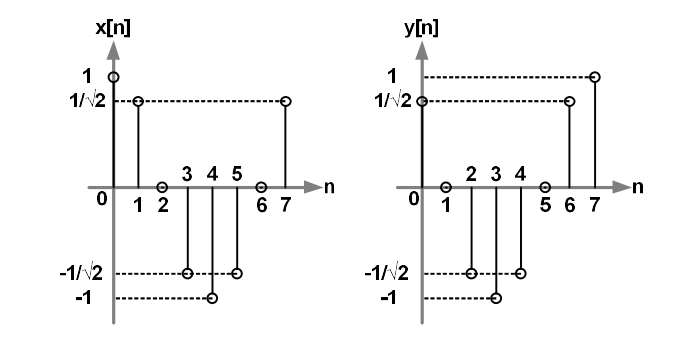
\includegraphics[width=0.5\columnwidth]{GATE/2022/BM/figs/q15.png}
% Placeholder for discrete signals image
\caption{}
\label{fig:bm-2022}
\end{figure}
\begin{enumerate}
\begin{multicols}{4}
\item $2\sqrt{2}$
\item $\frac{1}{2}\sqrt{2}$
\item $\frac{1}{2}$
\item $\frac{1}{\sqrt{2}}$
\end{multicols}
\end{enumerate}

